\section{The Curve of a Charged Droplet}
\hspace{0em}\indent Finding that the surface charge density of a charged droplet is constant, as shown in section (\ref{cpt:charged disc}), the charged droplet's height derived from this approach will serve as a simple test for its validity.

\citet{Fontelos2008_2} provides an equation in $r, \theta$ coordinates,  to derive a droplet's height from its curvature. Since we are using $x, y$ coordinates, we choose the equation from my supervisor's ``thin droplet problem" note, which is 
\[
h_{xx}=\Delta p -\frac{q^2}{2}\sigma_z^2
\]
\( h \) is the droplet's height, and integrating twice internally leads to the height, with some constants to be defined. For the charged droplet,
\begin{equation*}
    \begin{split}
        \sigma(\zeta)&=constant\Longrightarrow\sigma_z =\frac{1}{\sin \theta}=\frac{1}{\sqrt{1-x^2}}\\
        \Longrightarrow h&=\frac{\Delta P}{2}x^2-\frac{q^2}{2}\int\int\sigma_z^2\df x \df x +C_1 x + C_2\\
        &=\frac{\Delta P}{2}x^2-\frac{q^2}{2}\left(\frac{1-x}{2}\log(1-x)+\frac{1+x}{2}\log(1+x)\right) +C_1 x + C_2
    \end{split}
\end{equation*}
For the two constants, $C_1$, $C_2$, consider the boundary conditions:\vspace{-.5em}
\begin{itemize}
    \item Due to symmetry, the derivative of the height is $0$, at $x=0$.\vspace{-0.5em}
    \[
    h'(0)=0\Longrightarrow C_1\equiv 0
    \]
    \item The droplet sits on $x\in(-1, 1)$, hence\vspace{-0.5em}
    \[
       h(1)=0\Longrightarrow\frac{P}{2}-\frac{q^2}{2}\log2+C_2=0\Longrightarrow C_2=\frac{-P+q^2 \log2}{2}\vspace{-1em}
    \]
    \item We expect the droplet to sit above the substrate, meaning the height should always be greater than 0.\vspace{-0.5em}
     \[
        h\geq 0\Longrightarrow h(x=0)=C_2\geq 0
    \]
\end{itemize}\vspace{-0.5em}
Apply the boundary conditions, we find the height and the droplet curve, as in Figure (\ref{fig:height_charged}).
    \[
    h=\frac{\Delta P}{2}x^2+\frac{-P+q^2 \log2}{2}-\frac{q^2}{2}\left(\frac{1-x}{2}\log(1-x)+\frac{1+x}{2}\log(1+x)\right)\vspace{-1em}
    \]
\begin{figure}[H]
    \centering
    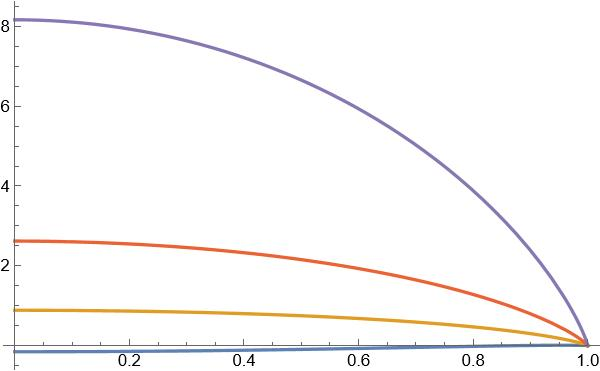
\includegraphics[width=1.\linewidth]{Figs/ho.jpg}
    \caption{\small The charged droplet's height/curve, with $q/\Delta P$ ratio 1, 2, 3, and 5. when $q/\Delta P=1$, the boundary is found below the substrate, which is not physically valid. Note that the peak of the curve rises as the charge in the droplet increases. Also note that, from physical properties, as the top of the droplet rises, its edges should contract, and thus will no longer be located at \(x = 1\). Therefore, the droplet curve obtained by this method is a self-similar solution, rather than a physical boundary.
}
    \label{fig:height_charged}
\end{figure}
\noindent The rising trend in the droplet shape follows the research findings\footnote{For the graph, see \href{https://news.mit.edu/2019/electrified-droplet-air-purification-0617}{"A droplet walks into an electric field"}.} from  \citet{BerozJ2019Droplet_shape_MIT} and FIG. 7, \citet{Fontelos2008}. This method may yield a physically meaningful height function.

